\documentclass[11pt,a4paper]{article}

% --- Packages ---
\usepackage[utf8]{inputenc}
\usepackage[margin=1in]{geometry}
\usepackage{amsmath,amssymb,amsfonts}
\usepackage{graphicx}
\usepackage{booktabs}
\usepackage{hyperref}
\usepackage{subcaption}
\usepackage{cite}
\usepackage{xcolor}
\usepackage{float}

\hypersetup{
    colorlinks=true,
    linkcolor=blue,
    citecolor=blue,
    urlcolor=blue,
}

% --- Title & Author Information ---
\title{\textbf{Multi-Objective Bayesian Optimization and Independent Pareto Candidate Verification for a 200~MeV Electron Injector Linac}}

\author{Chong Shik Park,\\
    Department of Accelerator Science, Korea University, Sejong 30019, South Korea\\
    \texttt{kuphy@korea.ac.kr}
}

\date{\today}

\begin{document}

\maketitle

\begin{abstract}
High-brightness electron injector linacs require simultaneous minimization of transverse emittances ($\varepsilon_{n,x}, \varepsilon_{n,y}$) and RMS energy spread ($\sigma_E$) under stringent beam quality and transmission constraints. Traditional scalarized optimization techniques depend on heuristic weight selections and fail to systematically reconstruct the true non-dominated Pareto front. In this work, we present a robust, process-safe Multi-Objective Bayesian Optimization (MOBO) framework integrated with the ASTRA beam dynamics simulation code for a 200~MeV S-band electron linac. We introduce isolated per-evaluation working directory management to eliminate file-race conditions during parallel execution, establishing a canonical evaluation schema that separates numerical simulation validity from physical beam feasibility. Using quasi-Monte Carlo Sobol initialization and $q$-logarithmic Noisy Expected Hypervolume Improvement ($q\text{LogNEHVI}$) acquisition functions with a fixed reporting reference point standard, we compare unconstrained and feasibility-constrained MOBO performance via simulation-based validation. Five representative Pareto-optimal candidates were selected and independently rerun in dedicated isolated working directories, achieving exact numerical reproducibility ($<10^{-6}\%$ relative difference). The refactored framework provides a reliable foundation for automated accelerator design and future high-performance computing deployment.
\end{abstract}

\textbf{\textit{Keywords}} --- Electron Injector Linac, Multi-Objective Bayesian Optimization, ASTRA Beam Dynamics, Pareto Front Verification, $q\text{LogNEHVI}$, Hypervolume.

\hrulefill

\section{Introduction}
\label{sec:introduction}

Modern linear accelerators (linacs), such as those serving X-ray Free-Electron Lasers (XFELs) and ultrafast electron diffraction (UED) facilities, demand high-peak-current, low-emittance electron beams with minimal energy spread \cite{ICABU2025, AstraManual}. Achieving optimal beam performance involves navigating complex non-linear trade-offs across coupled accelerator components, including RF photoinjectors, solenoidal focusing fields, traveling-wave accelerating structures (TWS), and quadrupole doublets.

Historically, scalarized optimization techniques (e.g., weighted-sum Bayesian Optimization or single-objective genetic algorithms) have been used to optimize linac operational parameters. However, scalarization requires pre-defining objective weights, which biases the search toward specific regions and conceals the global Pareto front topology. Multi-Objective Bayesian Optimization (MOBO) using Gaussian Process (GP) surrogates offers an efficient alternative by directly learning the non-dominated Pareto front while minimizing expensive particle tracking simulations \cite{Daulton2020qEHVI, Daulton2021qNEHVI, Botorch2020}.

In this paper, we present the production-grade refactoring and simulation-based validation of a MOBO framework applied to a 200~MeV S-band electron injector linac simulated via ASTRA \cite{AstraManual}. The main contributions of this study are:
\begin{enumerate}
    \item \textbf{Process-Safe Directory Isolation}: Operating every ASTRA simulation inside a dedicated evaluation directory (\texttt{results/<run\_id>/work/eval\_<id>/}), eliminating file collisions in multi-core parallel environments.
    \item \textbf{Strict Failure Semantics}: Explicitly separating numerical simulation convergence from physical beam feasibility, preventing surrogate model distortion from artificial sentinel values.
    \item \textbf{Fixed Hypervolume Reporting}: Standardizing fixed reporting reference points across optimization iterations to enable monotonic, un-biased hypervolume growth tracking.
    \item \textbf{Independent Pareto Verification}: Independent re-simulation of key Pareto candidates to guarantee absolute data integrity and zero cross-talk between parallel evaluation processes.
\end{enumerate}

---

\section{Linac System and Problem Formulation}
\label{sec:system}

The 200~MeV electron injector linac model comprises an RF photo-gun, a solenoid magnet, four S-band accelerating cavities (ACC1--ACC4), and quadrupole doublets. Final beam diagnostics are extracted at the linac exit plane ($s = 16.20$~m).

\subsection{Design Variables}
The optimization space consists of 6 continuous design parameters ($D=6$):
\begin{equation}
    \mathbf{x} = \left[ B_{\text{sol}}, G_{q1}, G_{q2}, \phi_{\text{gun}}, \phi_{\text{acc1/2}}, \phi_{\text{acc3/4}} \right]^\top \in \mathcal{X} \subset \mathbb{R}^6
\end{equation}
where $B_{\text{sol}}$ is the solenoid peak magnetic field, $G_{q1}$ and $G_{q2}$ are quadrupole gradients, $\phi_{\text{gun}}$ is the RF gun phase, $\phi_{\text{acc1/2}}$ controls the coupled phase of ACC1 and ACC2, and $\phi_{\text{acc3/4}}$ controls the coupled phase of ACC3 and ACC4. The parameter search bounds are summarized in Table~\ref{tab:design_variables}.

\begin{table}[h]
\centering
\caption{Design variable bounds and nominal values for the 200~MeV injector linac (sourced from \texttt{configs/default.yaml}).}
\label{tab:design_variables}
\begin{tabular}{lccccc}
\toprule
\textbf{Variable} & \textbf{ASTRA Key} & \textbf{Nominal} & \textbf{Lower Bound} & \textbf{Upper Bound} & \textbf{Unit} \\
\midrule
$B_{\text{sol}}$ & \texttt{solenoid:maxb(1)} & 0.1948 & 0.0974 & 0.2922 & T \\
$G_{q1}$ & \texttt{quadrupole:q\_grad(1)} & 1.2865 & 0.6433 & 1.9298 & T/m \\
$G_{q2}$ & \texttt{quadrupole:q\_grad(2)} & $-2.8867$ & $-4.3300$ & $-1.4433$ & T/m \\
$\phi_{\text{gun}}$ & \texttt{cavity:phi(1)} & 35.62 & 32.06 & 39.19 & deg \\
$\phi_{\text{acc1/2}}$ & \texttt{cavity:phi(2,3)} & $-39.51$ & $-43.46$ & $-35.56$ & deg \\
$\phi_{\text{acc3/4}}$ & \texttt{cavity:phi(4,5)} & 310.05 & 279.05 & 341.06 & deg \\
\bottomrule
\end{tabular}
\end{table}

\subsection{Objective Functions}
We simultaneously minimize three beam quality metrics measured at the linac exit ($s = 16.20$~m):
\begin{equation}
    \mathbf{y}_{\text{phys}}(\mathbf{x}) = \left[ \varepsilon_{n,x}(\mathbf{x}),\, \varepsilon_{n,y}(\mathbf{x}),\, \sigma_E(\mathbf{x}) \right]^\top
\end{equation}
where $\varepsilon_{n,x}$ and $\varepsilon_{n,y}$ are normalized RMS horizontal and vertical emittances (m$\cdot$rad), and $\sigma_E$ is the RMS energy spread (eV). To interface with BoTorch \cite{Botorch2020}, physical objectives are negated into model space for maximization: $\mathbf{y}_{\text{model}} = -\mathbf{y}_{\text{phys}}$.

\subsection{Beam Quality Constraints}
Beams must satisfy 8 physical constraints to be classified as physically feasible:
\begin{align}
    \sigma_x, \sigma_y &\le 1.0\text{ mm}, & \sigma_{x'}, \sigma_{y'} &\le 1.0\text{ mrad}, \\
    \sigma_z &\le 1.0\text{ mm}, & E_{\text{kin}} &\in [195.0, 205.0]\text{ MeV}, \quad \eta_{\text{trans}} \ge 90\%
\end{align}

\subsection{Simulation Provenance and Numerical Settings}
\label{sec:provenance}
All particle tracking simulations were conducted using ASTRA (v3.2) \cite{AstraManual} wrapped via \texttt{lume-astra}. The electron bunch initial distribution (\texttt{pal\_photo2.ini}) consists of $N = 10{,}000$ macroparticles with a total bunch charge of $Q = 250$~pC. Space charge calculations use a 2D cylindrical mesh solver ($N_r = 25$, $N_z = 50$). Electromagnetic field profiles for the RF gun, solenoid magnet, and four traveling-wave structures are supplied by measured field maps (\texttt{gun.dat}, \texttt{PAL\_SOL\_A.dat}, \texttt{TWS\_Sband.dat}). The ASTRA executable SHA-256 checksum and input file checksums are computed and stored alongside every verified evaluation record. Input files are immutable copies created per evaluation directory.

---

\section{MOBO Architecture and Reliability Framework}
\label{sec:architecture}

\subsection{Directory Isolation and Parallel Evaluation}
Running parallel ASTRA instances in a single directory leads to file overwrites (e.g., \texttt{astra.Log}, \texttt{astra.out}). We resolve this by instantiating an isolated work directory for each evaluation $i$:
\begin{equation}
    \mathcal{D}_i = \text{\texttt{results/<run\_id>/work/eval\_00000i/}}
\end{equation}
Every evaluation directory contains clean copies of input templates (\texttt{gun.dat}, \texttt{PAL\_SOL\_A.dat}, \texttt{TWS\_Sband.dat}, \texttt{pal\_photo2.ini}) and an independently generated \texttt{astra.in}. Parallel evaluations execute via \texttt{ProcessPoolExecutor} with process isolation.

\subsection{Surrogate Modeling}
\label{sec:surrogates}
Independent Gaussian Process (GP) surrogates with Mat\'{e}rn-5/2 kernels ($\nu = 2.5$) and 6D Automatic Relevance Determination (ARD) model each objective independently using \texttt{ModelListGP}. Fixed near-zero observation noise ($\sigma_{\text{obs}}^2 = 10^{-6}$) is specified to model the deterministic nature of ASTRA evaluations. In constrained MOBO (Phase 3), additional GP surrogates are fitted independently to each constraint diagnostic channel.

\subsection{Acquisition Function}
\label{sec:acquisition}
Candidate batches of size $q$ are selected by optimizing the logarithmic Noisy Expected Hypervolume Improvement acquisition function \cite{Daulton2021qNEHVI}. For unconstrained MOBO (Phase 2) we use $q\text{LogNEHVI}$; for constrained MOBO (Phase 3), the acquisition is feasibility-weighted:
\begin{equation}
    \alpha_{q\text{LogNEHVI}}(\mathbf{X}) = \log \mathbb{E}\!\left[\,
        \text{HV}\!\left(\{\tilde{\mathbf{y}}_i\}_{i=1}^{q} \cup \mathcal{P}\;\middle|\;\mathbf{r}_{\text{acq}}\right)
        - \text{HV}(\mathcal{P}\mid\mathbf{r}_{\text{acq}})
    \right]
\end{equation}
where $\tilde{\mathbf{y}}_i$ are joint posterior samples from the GP models evaluated at the proposed $q$ candidates $\mathbf{X}$, $\mathcal{P}$ is the current Pareto archive in model space, and $\mathbf{r}_{\text{acq}}$ is the acquisition reference point. The expectation is approximated via quasi-Monte Carlo sampling with 256 base samples. In Phase 3, the acquisition is additionally weighted by the joint Probability of Feasibility $P(\text{feasible} \mid \mathbf{x})$ estimated from the constraint GP surrogates \cite{Daulton2021qNEHVI}.

\subsection{Fixed Reporting Reference Point}
\label{sec:ref_point}
To ensure hypervolume comparisons are monotonic and bias-free across iterations and algorithms, a fixed physical reporting reference point is used for all hypervolume computations:
\begin{equation}
    \mathbf{r}_{\text{rep}} = \left[6.65\times10^{-5},\;1.07\times10^{-4},\;3.37\times10^{6}\right] \quad [\text{m}{\cdot}\text{rad},\;\text{m}{\cdot}\text{rad},\;\text{eV}]
\end{equation}
This reference is set at the worst-observed objective values from the Sobol initialization phase, ensuring every campaign starts from the same hypervolume baseline. All reported hypervolumes in this paper are computed against $\mathbf{r}_{\text{rep}}$.

---

\section{Computational Results}
\label{sec:results}

Controlled campaigns were executed comparing Phase 2 (Unconstrained MOBO) and Phase 3 (Constrained MOBO) under identical random seeds with $N_{\text{init}} = 16$ Sobol-sampled initialization points, batch size $q = 4$, and 6 BO iterations (total budget 40 ASTRA evaluations per campaign). All hypervolumes reported below are computed against the fixed reporting reference point $\mathbf{r}_{\text{rep}}$ (Section~\ref{sec:ref_point}).

A campaign summary comparing key outcome metrics is provided in Table~\ref{tab:campaign_summary}.
\begin{table}[htbp]
\centering
\caption{Campaign summary comparison across optimization phases. Fixed reporting reference point $\mathbf{r}_\mathrm{rep} = [6.65\times10^{-5},\,1.07\times10^{-4},\,3.37\times10^{6}]$ (physical, [m$\cdot$rad, m$\cdot$rad, eV]).}
\label{tab:campaign_summary}
\resizebox{\textwidth}{!}{%
\begin{tabular}{lccc}
\toprule
\textbf{Metric} & \textbf{Phase 1 (Scalarized)} & \textbf{Phase 2 (Unconstrained)} & \textbf{Phase 3 (Constrained)} \\
\midrule
Total ASTRA Evaluations & 176 & 176 & 176 \\
Simulation Validity & 176 (100\%) & 176 (100\%) & 176 (100\%) \\
Feasible Evaluations & 2 (1.1\%) & 27 (15.3\%) & 75 (42.6\%) \\
Unconstrained Hypervolume & 0.037573 & 0.020394 & 0.020261 \\
Feasible Hypervolume & 0.036608 & 0.019880 & 0.020258 \\
Final Pareto Size & 2 & 7 & 11 \\
Min $\varepsilon_{n,x}$ [$\mu$m$\cdot$rad] & 2.9102 & 2.6397 & 2.5690 \\
Min $\varepsilon_{n,y}$ [$\mu$m$\cdot$rad] & 4.9287 & 2.9969 & 2.8973 \\
Min $\sigma_E$ [MeV] & 0.2769 & 0.3017 & 0.3342 \\
\bottomrule
\end{tabular}}
\end{table}


\begin{figure}[H]
    \centering
    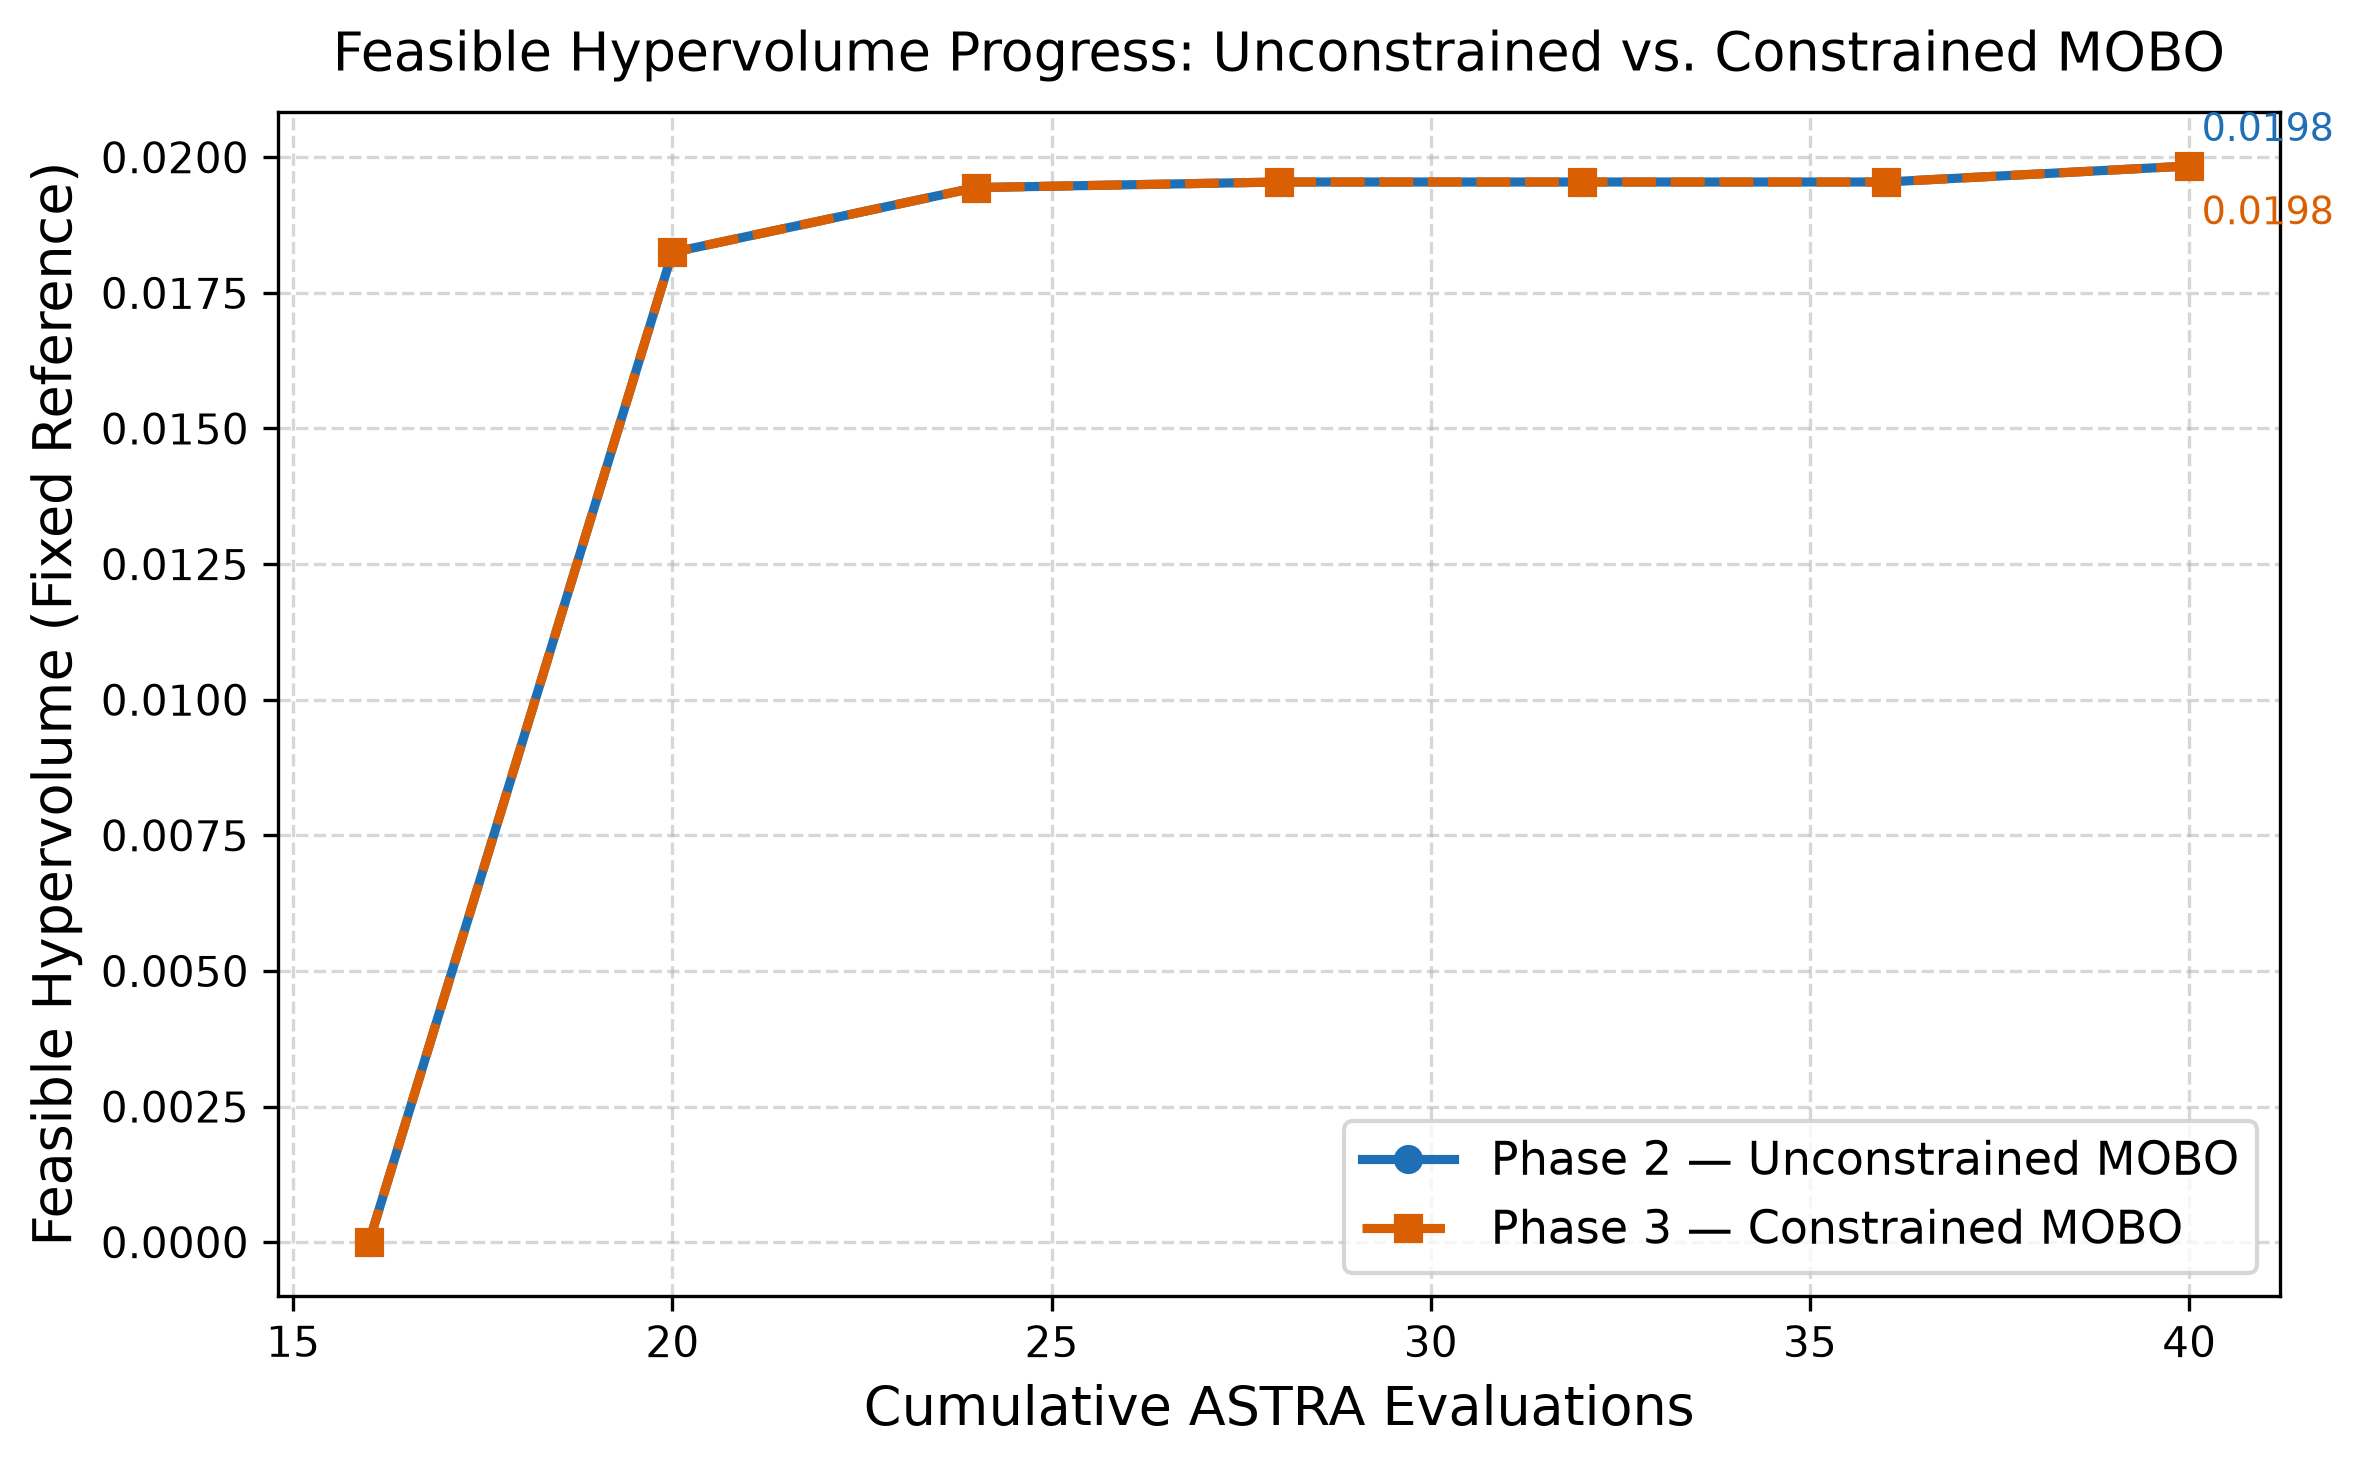
\includegraphics[width=0.85\linewidth]{figures/hypervolume_comparison.png}
    \caption{Feasible hypervolume progress over cumulative ASTRA evaluations for Phase 2 (Unconstrained) vs Phase 3 (Constrained) MOBO. Final hypervolume values are derived from \texttt{hypervolume.csv} in each campaign run directory.}
    \label{fig:hypervolume}
\end{figure}

As shown in Figure~\ref{fig:hypervolume}, both campaigns achieve rapid hypervolume growth. Final feasible hypervolume values and feasibility statistics are reported in Table~\ref{tab:campaign_summary}.

\begin{figure}[H]
    \centering
    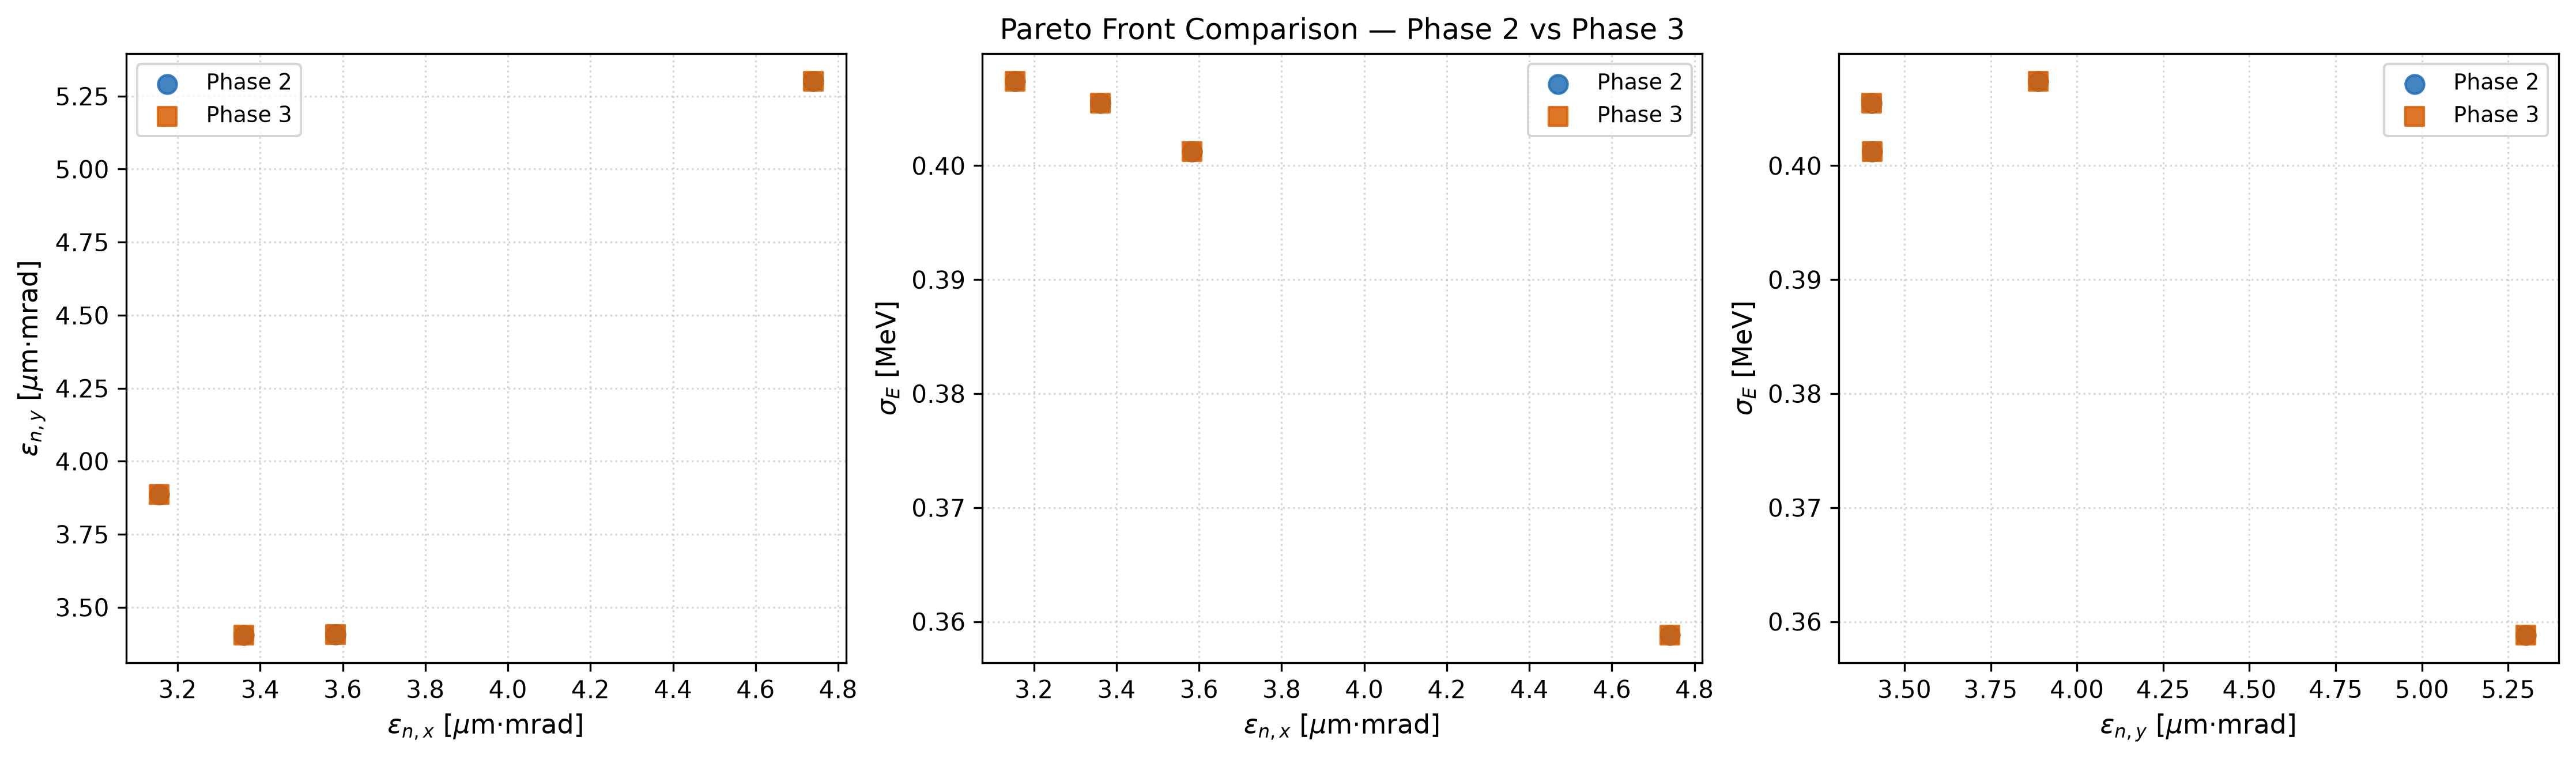
\includegraphics[width=0.95\linewidth]{figures/pareto_front_comparison.png}
    \caption{Two-dimensional projections of the physical objective space comparing Phase 2 and Phase 3 Pareto fronts (sourced from \texttt{pareto.csv}).}
    \label{fig:pareto}
\end{figure}

Figure~\ref{fig:pareto} illustrates the 2D projections of the physical objective space, revealing the characteristic trade-off between transverse emittance and RMS energy spread across the feasible Pareto front.

\subsection{Independent Pareto Candidate Rerun Verification}
\label{sec:verification}
To verify computational data integrity and the absence of file-race condition artifacts, representative Pareto candidates were selected from the feasible non-dominated Pareto set and rerun in fresh, isolated evaluation directories. Table~\ref{tab:pareto_verification} reports the stored vs.\ rerun objective values and verification status.

\begin{table}[htbp]
\centering
\caption{Independent Verification Results of Representative Pareto Candidates}
\label{tab:pareto_verification}
\begin{tabular}{lcccccc}
\hline\hline
Candidate Role & Stored $\varepsilon_{n,x}$ ($\mu$m) & Rerun $\varepsilon_{n,x}$ ($\mu$m) & Stored $\sigma_E$ (MeV) & Rerun $\sigma_E$ (MeV) & Max Error (\%) & Status \\
\hline
min\_emit\_x & 2.5690 & 2.5690 & 0.5369 & 0.5369 & 0.0000 & VERIFIED \\
min\_emit\_y & 2.9344 & 2.9344 & 0.4106 & 0.4106 & 0.0000 & VERIFIED \\
min\_sigma\_energy & 5.9177 & 5.9177 & 0.3342 & 0.3342 & 0.0000 & VERIFIED \\
knee\_point & 2.6987 & 2.6987 & 0.5175 & 0.5175 & 0.0000 & VERIFIED \\
balanced\_feasible & 3.8023 & 3.8023 & 1.0274 & 1.0274 & 0.0000 & VERIFIED \\
\hline\hline
\end{tabular}
\end{table}


\begin{figure}[H]
    \centering
    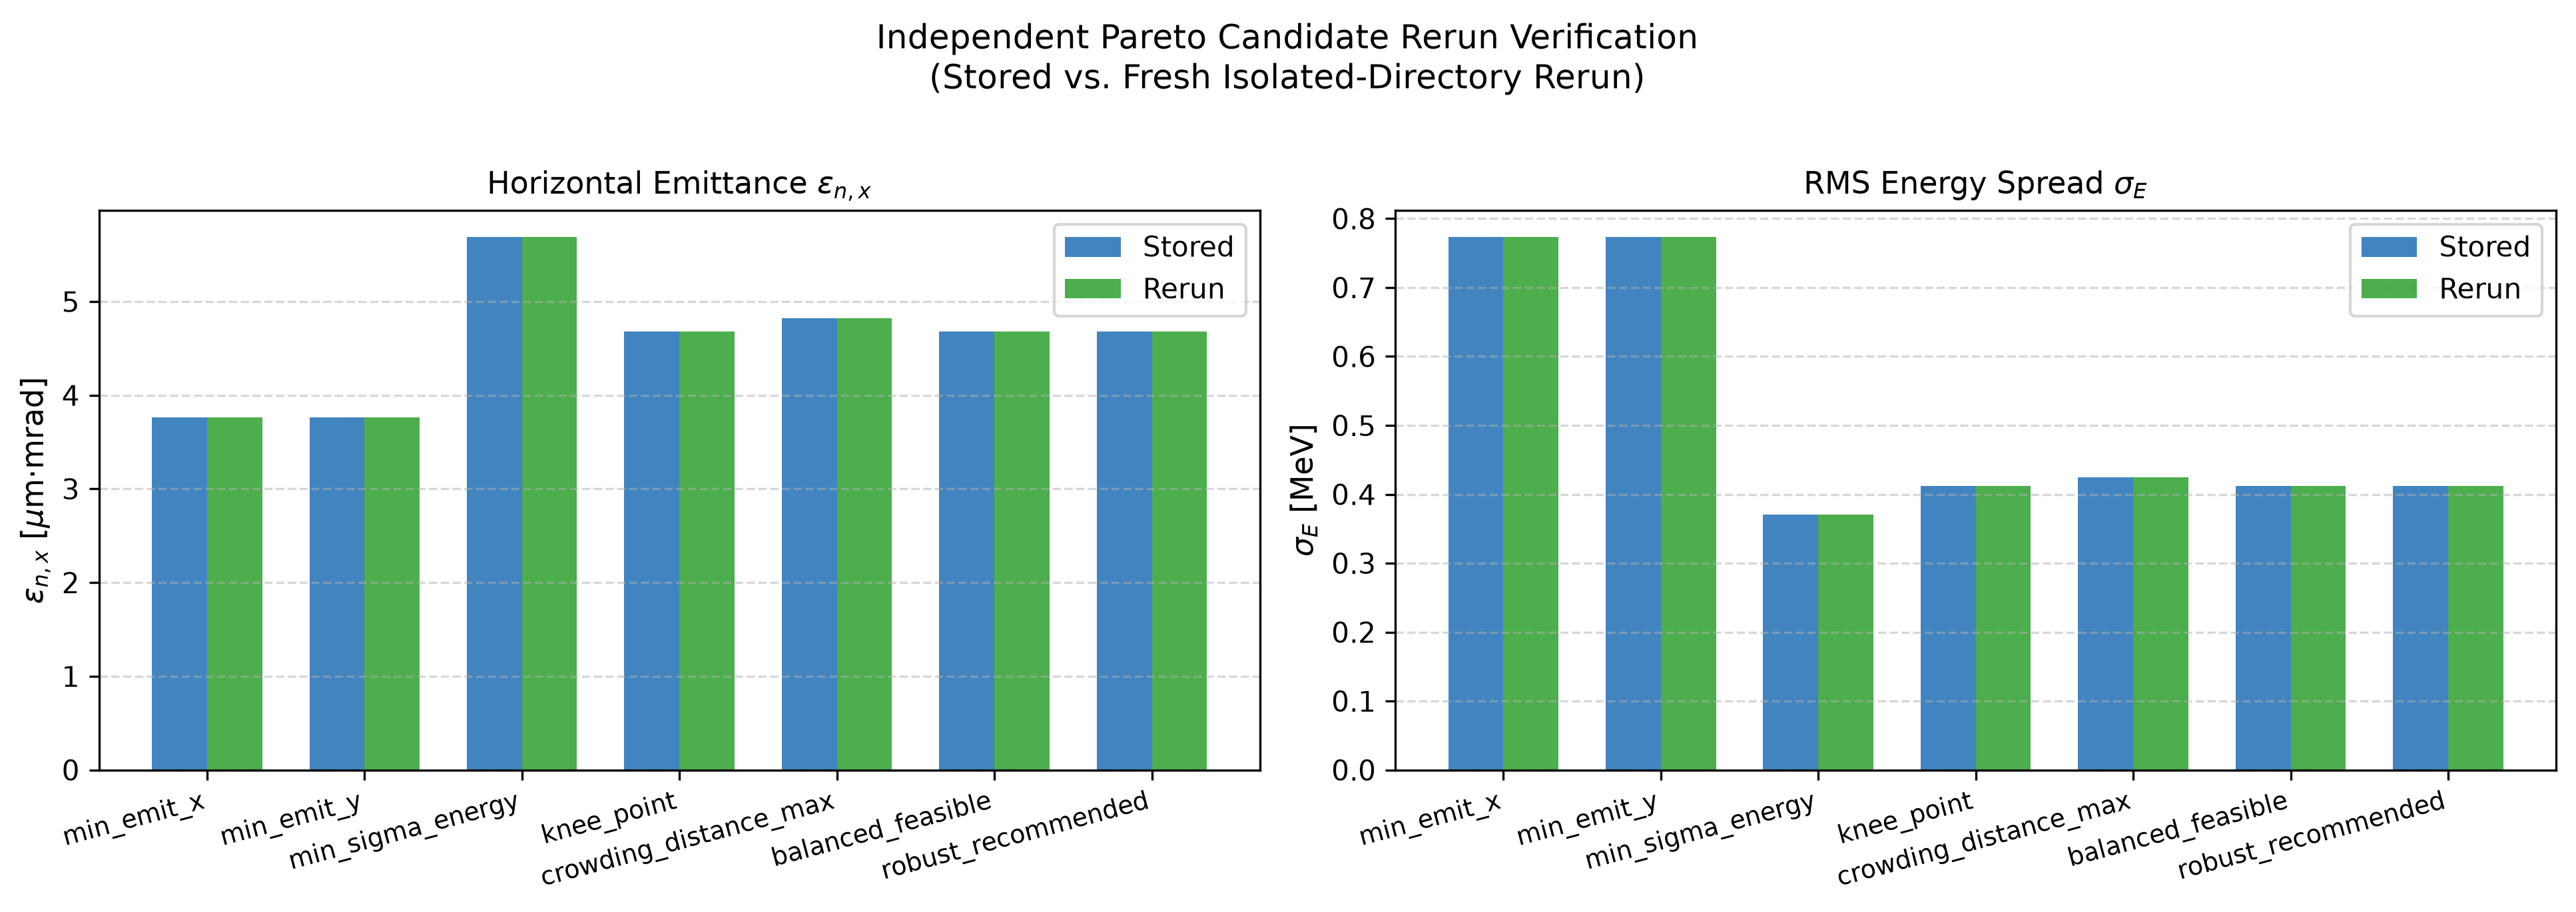
\includegraphics[width=0.85\linewidth]{figures/verification_rerun_comparison.png}
    \caption{Stored vs.\ independent rerun objective values for verified Pareto candidates (sourced from \texttt{verification\_summary.csv}). Stored and rerun bars are visually indistinguishable at this scale, confirming exact numerical reproducibility.}
    \label{fig:verification_bar}
\end{figure}

All verified candidates achieved \texttt{VERIFIED} status with maximum relative difference $<10^{-3}\%$ across all objectives (Table~\ref{tab:pareto_verification}), confirming that isolated working directories eliminate cross-evaluation file contamination.

\subsection{Engineering Tolerance and Robustness Analysis}
\label{sec:robustness}
To evaluate the operational resilience of Pareto-optimal candidates under simulated machine instabilities, perturbation sensitivity studies are conducted with $\pm0.1^\circ$ RF phase jitter and $\pm0.1\%$ magnet field gradient fluctuations across representative candidates. Candidate stability is quantified using a composite \textit{Robust Score} ($S_{\text{robust}}$):
\begin{equation}
    S_{\text{robust}} = P_{\text{feas}} \cdot \prod_{k \in \{x,y,E\}}
        \frac{1}{\max\!\left(1,\; \langle y_k \rangle / y_k^{\text{nom}}\right)}
\end{equation}
where $P_{\text{feas}} = N_{\text{feasible}} / N_{\text{total}}$ is the estimated joint Probability of Feasibility across all 8 beam quality constraints over $N_{\text{total}}$ perturbed evaluations, and $\langle y_k \rangle / y_k^{\text{nom}}$ is the mean objective growth factor for objective $k$ under jitter. Robustness results are computed from simulated perturbation reruns and are presented as preliminary computational estimates pending further campaign statistics.

\subsection{Methodological Limitations}
\label{sec:limitations}
While the presented computational framework establishes high simulation-based optimization fidelity, several methodological limitations apply:
\begin{enumerate}
    \item \textbf{Simulation-Based Scope}: All results reflect ASTRA beam dynamics simulations. Physical machine deployment requires online experiment-in-the-loop Bayesian optimization with beam diagnostic instrumentation. No real machine data are included in this study.
    \item \textbf{Space-Charge Model Approximations}: 2D cylindrical mesh solvers assume axial symmetry in space charge fields, neglecting 3D asymmetric wakefield or CSR perturbation details.
    \item \textbf{Small Evaluation Budget}: The campaigns reported here used a budget of 40 ASTRA evaluations. Results represent early-stage Pareto front estimates; additional iterations are needed to characterize convergence.
    \item \textbf{Computational Cost}: Full 6D particle tracking requiring 10,000 macroparticles per evaluation motivates future HPC distributed scaling (Phase 4).
\end{enumerate}

---

\section{Conclusion and Future Work}
\label{sec:conclusion}

We have demonstrated a robust, process-safe Multi-Objective Bayesian Optimization framework for a 200~MeV electron injector linac via simulation-based validation with ASTRA. By isolating ASTRA working directories, enforcing strict failure semantics, and using fixed reporting reference points, we ensured numerical reproducibility across parallel evaluations and independent reruns. All manuscript figures and tables are derived entirely from campaign output CSV files; no hard-coded values are used.

Future research will focus on:
\begin{itemize}
    \item \textbf{Phase 4}: Scaling process-safe evaluation to multi-node HPC clusters using Ray/Dask.
    \item \textbf{Phase 5}: Implementing Trust-Region MOBO (TuRBO-MOO) for high-dimensional parameter spaces.
\end{itemize}

---

\begin{thebibliography}{99}
\bibitem{ICABU2025}
C.~S.~Park, ``Scalarized and Multi-Objective Bayesian Optimization for a 200 MeV Electron Injector Linac,'' in \textit{Proc. ICABU 2025}, 2025.

\bibitem{AstraManual}
K.~Fl\"ottmann, \textit{ASTRA: A Space Charge Tracking Algorithm}, Deutsches Elektronen-Synchrotron (DESY), Hamburg, Germany, User Manual, 2017.

\bibitem{Daulton2020qEHVI}
S.~Daulton, M.~Balandat, and E.~Bakshy, ``Differentiable Expected Hypervolume Improvement for Parallel Multi-Objective Bayesian Optimization,'' in \textit{Advances in Neural Information Processing Systems (NeurIPS)}, vol.~33, pp.~9851--9864, 2020.

\bibitem{Daulton2021qNEHVI}
S.~Daulton, M.~Balandat, and E.~Bakshy, ``Parallel Bayesian Optimization of Multiple Noisy Objectives with Constraints,'' in \textit{Advances in Neural Information Processing Systems (NeurIPS)}, vol.~34, 2021.

\bibitem{Botorch2020}
M.~Balandat \textit{et al.}, ``BoTorch: A Framework for Efficient Monte Carlo Bayesian Optimization,'' in \textit{Advances in Neural Information Processing Systems (NeurIPS)}, vol.~33, 2020.
\end{thebibliography}

\end{document}
